\chapter{Sobre simetrías en las entradas de los polinomios de Legendre discretos}
\label{section: sobre simetrias en las entradas de los poliomios discretos de Legendre}
Puesto que planeamos implementar computacionalmente
las bases de Legendre discretas, es de utilidad 
buscar simetrías en las entradas de los vectores que las 
componen, pues esto puede reducir significativamente
el número de operaciones requeridas para el cálculo 
de bases de este tipo.
Ya los valores calculados
en la subsección 
\ref{formulas explicitas para Ln con n de 2 hasta 6}
sugieren 
la existencia de tales simetrías en las entradas 
de los vectores de la forma $\cali{L}^{n,k} \in \IR^{n}$
que, recordamos, se han definido en 
\ref{def: base de Legendre discreta}.


\begin{figure}[H] \label{fig: simetrias entradas Legendre}
\centering\captionsetup{format = hang}
	\begin{measuredfigure}
		\includegraphics[scale=1.7]{simetrias_Legendre} 
		\caption{ 
		Se muestran en la tabla las bases de Legendre
		discreta de dimensiones entre dos y seis. 		
		Para las dimensiones $n$ marcadas
		puede apreciarse que, en el vector,
		 $\cali{L}^{n,k} = \left( \cali{L}^{n,k}_{m} \right)_{m=0}^{n-1}$,
		las entradas a la derecha son iguales a las de la izquierda,
		con un cambio de signo que depende del
		grado $k$ del polinomio discreto de Legendre.}
		\label{fig: simetrias entradas Legendre}
 	\end{measuredfigure} 
 \end{figure}

A pesar de que, a estas alturas, ya contamos
con expresiones para los vectores $\cali{L}^{n,k}$
(para cualesquiera entero $n \geq 2$ y $0 \leq k \leq n-1$,
c.f. teorema \ref{teo: expresión analítica de BON de Legendre}),
no será usando estas que podremos demostrar que, en efecto,
se tienen las simetrías sugeridas en la figura
~\ref{fig: simetrias entradas Legendre}.
Conviene
usar una de las múltiples definiciones iniciales
que dimos para la base $\cali{L}^{n}$, a saber, una
que involucre discretizaciones puntuales de polinomios 
que dé lugar a vectores $w_{k}$ que ya presenten 
este tipo de simetrías; por lo demostrado en secciones anteriores,
no perdemos generalidad al hacer esto. 


%Tabla para n=2,3,4
\begin{center}
\begin{tabular}{ c c c c c c }
k $\backslash$ n & 2 & 3 & 4   \\ 
\hline

0 & $\left(
\frac{1}{\sqrt{2}}, \frac{1}{\sqrt{2}}\right)$ & 
$\left(\frac{1}{\sqrt{3}}, \frac{1}{\sqrt{3}}, \frac{1}{\sqrt{3}} \right)$ & 
$\left(\frac{1}{2}, \frac{1}{2}, \frac{1}{2}, \frac{1}{2} \right)$ \\ 
1 & $\left(-\frac{1}{\sqrt{2}}, \frac{1}{\sqrt{2}}\right)$ & 
$\left(-\frac{1}{\sqrt{2}}, 0, \frac{1}{\sqrt{2}} \right) $ & 
$\left(-\frac{3}{2\sqrt{5}}, -\frac{1}{2\sqrt{5}}, \frac{1}{2\sqrt{5}}, \frac{3}{2\sqrt{5}} \right)$  \\ 
2 & $---$ & $\left(\frac{1}{\sqrt{6}}, -\sqrt{\frac{2}{3}}, \frac{1}{\sqrt{6}} \right) $ & 
$\left(\frac{1}{2}, -\frac{1}{2}, -\frac{1}{2}, \frac{1}{2} \right)$ \\ 
3 & $---$ & $---$ & 
$\left(-\frac{1}{2\sqrt{5}}, \frac{3}{2\sqrt{5}}, -\frac{3}{2\sqrt{5}}, \frac{1}{2\sqrt{5}} \right)$  \\ 
\end{tabular}
\end{center} 
 
%Tabla para n=5,6
\begin{center}
\begin{tabular}{ c c c c c c }
k $\backslash$ n & 5 & 6  \\ 
\hline
0 & 
$\left(\frac{1}{\sqrt{5}}, \frac{1}{\sqrt{5}}, \frac{1}{\sqrt{5}},
\frac{1}{\sqrt{5}}, \frac{1}{\sqrt{5}} \right)$ 
& $\left(\frac{1}{\sqrt{6}}, \frac{1}{\sqrt{6}}, \frac{1}{\sqrt{6}},
\frac{1}{\sqrt{6}}, \frac{1}{\sqrt{6}}, \frac{1}{\sqrt{6}} \right)$ \\ 
1 &  
$\left(-\sqrt{\frac{2}{5}}, -\frac{1}{\sqrt{10}}, 0,
\frac{1}{\sqrt{10}}, \sqrt{\frac{2}{5}} \right)$  & 
$\left(-\sqrt{\frac{5}{14}}, -\frac{3}{\sqrt{70}}, -\frac{1}{\sqrt{70}},
\frac{1}{\sqrt{70}}, \frac{3}{\sqrt{70}}, \sqrt{\frac{5}{14}} \right)$ \\ 
2 & 
$\left(\sqrt{\frac{2}{7}}, -\frac{1}{\sqrt{14}}, -\sqrt{\frac{2}{7}},
-\frac{1}{\sqrt{14}}, \sqrt{\frac{2}{7}} \right)$ 
& $\left(\frac{5}{2\sqrt{21}}, -\frac{1}{2\sqrt{21}}, -\frac{2}{\sqrt{21}},
-\frac{2}{\sqrt{21}}, -\frac{1}{2\sqrt{21}}, \frac{5}{2\sqrt{21}} \right)$ \\ 
3 & 
$\left(-\frac{1}{\sqrt{10}}, \sqrt{\frac{2}{5}}, 0,
-\sqrt{\frac{2}{5}}, \frac{1}{\sqrt{10}} \right)$ &
$\left(-\frac{\sqrt{5}}{6}, \frac{7}{6\sqrt{5}}, \frac{2}{3\sqrt{5}},
-\frac{2}{3\sqrt{5}}, -\frac{7}{6\sqrt{5}}, \frac{\sqrt{5}}{6} \right)$ \\ 
4 & $\left(\frac{1}{\sqrt{70}}, -\frac{2\sqrt{2}}{\sqrt{35}}, 
\frac{3\sqrt{2}}{\sqrt{35}},
-\frac{2\sqrt{2}}{\sqrt{35}}, \frac{1}{\sqrt{70}} \right) $ & 
$\left(\frac{1}{2\sqrt{7}}, -\frac{3}{2\sqrt{7}}, \frac{1}{\sqrt{7}},
\frac{1}{\sqrt{7}}, -\frac{3}{2\sqrt{7}}, \frac{1}{2\sqrt{7}} \right)$ \\ 
5 & $---$ & 
$\left(-\frac{1}{6\sqrt{7}}, \frac{5}{6\sqrt{7}}, -\frac{5}{3\sqrt{7}},
\frac{5}{3\sqrt{7}}, -\frac{5}{6\sqrt{7}}, \frac{1}{6\sqrt{7}} \right)$ 
\end{tabular}
\end{center}

\begin{figure}[H]
	\sidecaption{
	En la figura se ilustran los polinomios y las
		mallas uniformes que escogeremos cuando las dimensiones sean
		$n=4$ (dimensión par) y $n=7$ (dimensión impar). Observe que
		las discretizaciones obtenidas con estas elecciones presentan
		las simetrías descritas en la figura 
		\ref{fig: simetrias entradas Legendre}.
	\label{fig: simetrias polinomiales}
	}
	\centering
	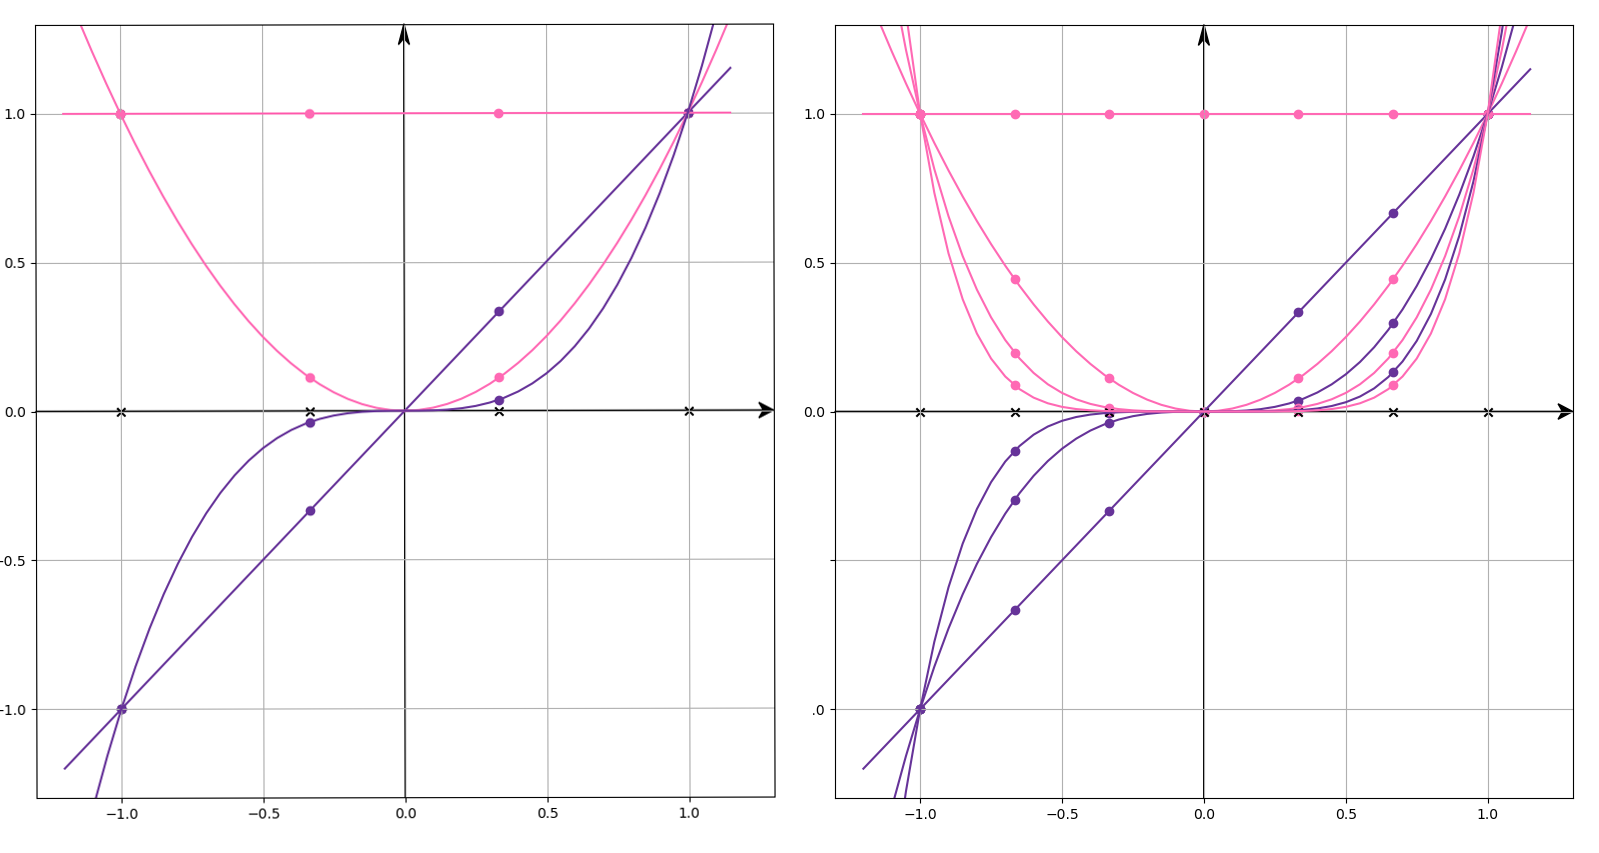
\includegraphics[scale=0.8]{10Dic_1} 
\end{figure}	


\subsection{Estudio para dimensiones impares}
A lo largo de esta subsección vamos a fijar
una dimensión 
$n \in \IN$ impar; digamos que

\begin{equation}
\label{eq1: 19En}
n=2N +1 \hspace{0.2cm} \text{ con } N \in \IN.
\end{equation}
Estudiemos las simetrías presentes en las entradas
de los vectores $\cali{L}^{n,k}$, con $0 \leq k \leq n-1$.

Para la discusión que sigue será conveniente definir
a los siguientes subconjuntos de $\IR^{n}$;

\begin{equation}
\label{eq0: 5Dic}
S_{+}:= \{ x=(x_{m})_{m=0}^{n-1} \in \IR^{n} \hspace{0.2cm} 
| \hspace{0.2cm} \forall  
\hspace{0.1cm}
0 \leq m \leq N-1 : \hspace{0.2cm} x_{m}= x_{2N-m}\},
\end{equation}
a cuyos elementos los denominaremos
\textbf{señales simétricas} de dimensión $n$,
\begin{equation}
\label{eq1: 5Dic}
S_{-}:= \{ x=(x_{m})_{m=0}^{n-1}  \in \IR^{n}
\hspace{0.2cm} |
\hspace{0.2cm} \forall  
\hspace{0.1cm}
0 \leq m \leq N-1 : \hspace{0.2cm} x_{m}= -x_{2N-m}\},
\end{equation}
llamando \textbf{señales antisimétricas} de dimensión $n$
a sus elementos, 
y también a
\begin{equation}
\label{eq2: 19En}
S_{-,0}:= \{ x=(x_{m})_{m=0}^{n-1}| \hspace{0.2cm} \forall  
\hspace{0.1cm}
0 \leq m \leq N-1 : \hspace{0.2cm} x_{m}= -x_{2N-m} 
\hspace{0.2cm} \text{y } x_{N}=0
\},
\end{equation}
el conjunto de señales antisimétricas de dimensión $n$
y entrada central nula.

Las siguientes dos observaciones se siguen de inmediato.

\begin{obs}
\label{obs: espacios de senales sim y antisim}
Sea $n$ como en \eqref{eq1: 19En}. 
Los conjuntos definidos en 
\eqref{eq0: 5Dic}, \eqref{eq1: 5Dic} y  \eqref{eq2: 19En}
son subespacios de $\IR^{n}$.
\end{obs}

\begin{obs}
\label{obs: pertenencia}
Sea $n$ como en \eqref{eq1: 19En}. 
Sea $\cali{P}$ la malla
uniforme de $n$ puntos con puntos extremos $-1$ y $1$.
Para toda $0 \leq k \leq n-1$, sean
las potencias básicas $f_{k}(t)=t^{k}$ y los vectores
\begin{equation}
\label{eq4: 10Dic}
w_{k}=(w_{k,m})_{m=0}^{n-1} := \Omega_{n, \cali{P}}(f_{k}),
\end{equation}
donde $\Omega_{n, \cali{P}}$ es el operador definido en 
\ref{def: operador de discretizacion puntual}.
Para toda $0 \leq k \leq n-1$ se tiene que
\begin{itemize}
\item $w_{k} \in S_{+}$ si $k$ es par, y
\item $w_{k} \in S_{-,0}$ si $k$ es impar,
\end{itemize}
donde $S_{+}$ y $S_{-,0}$ son como en 
\eqref{eq0: 5Dic} y \eqref{eq2: 19En}.
\end{obs}

Es fácil establecer la perpendicularidad entre
señales simétricas con señales antisimétricas.
Hacemos esto a continuación

\begin{lema}
\label{lema: ortogonalidad entre sim y antisim}
Sean $S_{+}$ y $S_{-,0}$ como en 
\eqref{eq0: 5Dic} y \eqref{eq2: 19En}. Para cualesquiera 
$u \in S_{+}$ y $v \in S_{-,0}$ se tiene que
$\langle u, v \rangle=0$.
\end{lema}
\noindent
\textbf{Demostración.}
Digamos que 
\begin{equation*}
u=(a_{0}, \ldots , a_{N-1}, a_{N}, a_{N-1}, \ldots a_{0}),
\end{equation*}
y que 
\begin{equation*}
v=(b_{0}, \ldots , b_{N-1}, 0, b_{N-1}, \ldots b_{0}).
\end{equation*}
Se calcula directamente que 

\[
\langle u, v \rangle = \suma{m=0}{N-1}{a_{m} \cdot b_{m}} + a_{N} \cdot 0
-\suma{m=0}{N-1}{a_{m} \cdot b_{m}} =0.
\]

\QEDB
\vspace{0.2cm}

\vspace{1cm}

\begin{comment}
{\Large{
$\cali{L}^{n,k}= \left( 
\cali{L}^{n,k}_{0}, 
\cali{L}^{n,k}_{1},
\cdots,
\cali{L}^{n,k}_{N-1},
\cali{L}^{n,k}_{N},  
\cali{L}^{n,k}_{N+1},
\cdots,
\cali{L}^{n,k}_{2N-1},
\cali{L}^{n,k}_{2N}
 \right)$.
 }}

 


{\Large{input}}
{\Large{$n=5$}}
{\Large{output}}
{\Large{$\longrightarrow$}}

{\large{
\begin{align*}
[[0.4472,0.4472,0.4472,0.4472,0.4472], \\
[-0.6324, -0.3162,0,0.3162,0.6324], \\
[0.5345, -0.2673, -0.5345, -0.2673, 0.5345], \\
[-0.3162, 0.6324, 0, -0.6324, 0.3162], \\
[0.1195, -0.4781, 0.7171, -0.4781, 0.1195] 
]
\end{align*}
}}
\end{comment}


\vspace{1cm}

Ya tenemos todo lo necesario para demostrar que las
señales de Legendre discretas de dimensión $n$ y grado
par son simétricas, mientras que las de grado
impar son antisimétricas.

\begin{teo}
\label{prop: simetrias en dimensiones impares}
\textbf{(Sobre simetrías
en los polinomios discretos de Legendre de dimensión impar)}. 
Sea $n \in \IN$ como en \eqref{eq1: 19En}.
Sea $0 \leq k \leq n-1$ y
considere al vector $\cali{L}^{n,k}=(\cali{L}^{n,k}_{m})_{m=0}^{n-1}$
como se ha definido en \eqref{def: base de Legendre discreta}. 
Se tiene que 
\begin{itemize}
\item $\cali{L}^{n,k} \in S_{+}$ si $k$ es par, y que
\item $\cali{L}^{n,k} \in S_{-,0}$ si $k$ es impar,
\end{itemize}
es decir, que para toda $0 \leq m \leq N-1$ se tiene que
\begin{itemize}
\item $\cali{L}^{n,k}_{m} = \cali{L}^{n,k}_{2N-m}$ si $k$ es par y
\item $\cali{L}^{n,k}_{m} = -\cali{L}^{n,k}_{2N-m}$ y 
$\cali{L}^{n, k}_{N}=0$ si $k$ es impar.
\end{itemize}
\end{teo}
\begin{figure}[H]
\centering\captionsetup{format = hang}
	\begin{measuredfigure}
		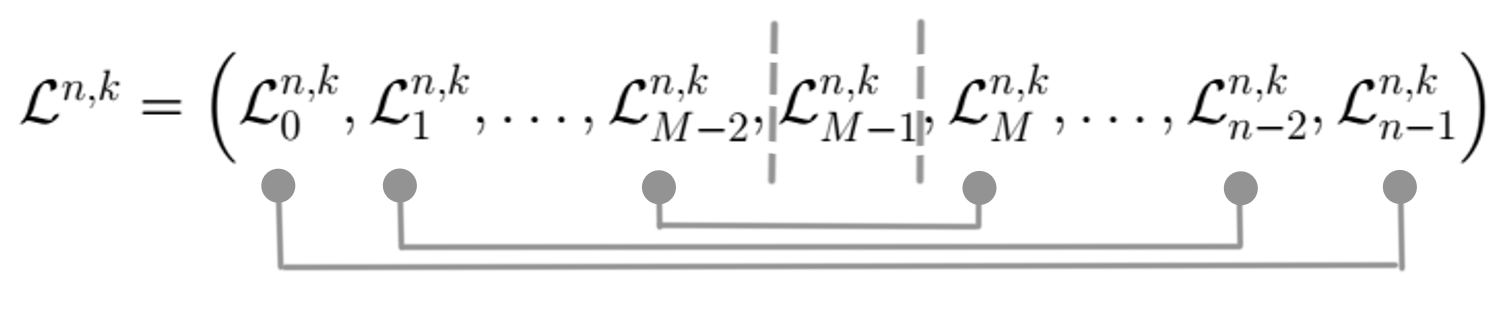
\includegraphics[scale=0.7]{simetria1} 
		\caption{Fijadas una dimensión impar $n=2N+1$ 
		y un grado $0 \leq k \leq n-1$,
		en esta proposición se da una relación simple entre las parejas 
		de entradas de $\cali{L}^{n,m}$ con índices $m$ y $2N-m$ 
		(donde los índices $0 \leq m \leq N-1$ son los de las primeras
		$N$ entradas).}
 	\end{measuredfigure}
 \end{figure}

\noindent
\textbf{Demostración.}
Sean los vectores $w_{k}$ como en la observación 
\ref{obs: pertenencia}.
Según lo demostrado en la subsección \TODO{ref}, si
\[
\{ \overline{\eta}_{k} : \hspace{0.2cm} 0 \leq k \leq n-1 \}
\]
es la base de $\IR^{n}$ que se obtiene al ortogonalizar 
con el proceso de Gram-Schmidt a la base
\[
\{ w_{k} : \hspace{0.2cm} 0 \leq k \leq n-1 \}
\]
de $\IR^{n}$,
o sea, si 

\begin{equation}
\label{eq3: 19En}
\overline{\eta}_{0}= w_{0},
\end{equation}
y si

\begin{equation}
\label{eq3: 19En}
\forall \hspace{0.1cm} 1 \leq k \leq n-1: 
\hspace{0.2cm}
\overline{\eta}_{k}= w_{k}-
\suma{j=0}{k-1}{
\frac{\langle w_{k}, \overline{\eta}_{j} \rangle}
{\langle \overline{\eta}_{j}, \overline{\eta}_{j} \rangle}\overline{\eta}_{j},
}
\end{equation}


\noindent
entonces, para toda $0 \leq k \leq n-1$ tenemos la relación 
\[
\cali{L}^{n,k}= \frac{1}{||\overline{\eta}_{k}||} \cdot \overline{\eta}_{k};
\]
en particular, los vectores $\cali{L}^{n,k}$ y 
$\overline{\eta}_{k}$ son múltiplos escalares uno del otro.

Afirmamos que ocurre que
$\overline{\eta}_{k} \in S_{+}$ (resp. que
$\overline{\eta}_{k} \in S_{-,0}$) si $k$ es par
(resp. impar); por ser $S_{+}$
y $S_{-,0}$ cerrado bajo multiplicación
por escalares (c.f. observación 
\ref{obs: espacios de senales sim y antisim}),
si logramos demostrar esta afirmación podremos concluir lo deseado.


Procedemos a demostrar esto por inducción sobre $k$.

\begin{itemize}

\item (Base de inducción) según la igualdad
\eqref{eq3: 19En} y la observación 
\ref{obs: pertenencia}, la afirmación 
es trivialmente cierta para $k=0$, el menor grado par.
Considere ahora a $k=1$, el menor grado impar. Según 
\eqref{eq3: 19En}, 
\begin{equation}
\label{eq5: 19En}
\overline{\eta}_{1}= w_{1}
- \frac{\langle w_{1}, \overline{\eta}_{0} \rangle}
{\langle \overline{\eta}_{0}, \overline{\eta}_{0} \rangle}\overline{\eta}_{0};
\end{equation}
De la observación 
\ref{obs: pertenencia} y el lema
\ref{lema: ortogonalidad entre sim y antisim} se sigue
que el producto punto $\langle w_{1}, \overline{\eta}_{0} \rangle$
es cero; sustituyendo esto en \eqref{eq5: 19En}
se infiere que 
\[
\overline{\eta}_{1} = w_{1} + 0 \cdot \overline{\eta}_{0}=
w_{1} \in S_{-}.
\]
Digamos pues que

\[
\overline{\eta}_{1} = 
(a_{0}, \ldots , a_{N-1}, a_{N}, -a_{N-1}, \ldots , -a_{0} );
\]
para completar la base de inducción debemos de mostrar
que $a_{N}$, la entrada central de $\overline{\eta}_{1}$,
es cero. Según \eqref{eq2: 19En} y
la definición del polinomio discreto $w_{0}$, 
$\overline{\eta}_{0}$ es el vector constante uno de $\IR^{n}$;
ahora bien, puesto que $\overline{\eta}_{0}$
y $\overline{\eta}_{1}$
son ortogonales entre sí, llegamos, como queríamos, a que

\[
0 = \langle \overline{\eta}_{0}, \overline{\eta}_{1}\rangle
= \suma{m=0}{n-1}{a_{m}} = 
\suma{m=0}{N-1}{a_{m}} +a_{N} -
\suma{m=0}{N-1}{a_{m}} = a_{N}.
\]



\item (Paso inductivo) sea $0 \leq k \leq n-1$ par, y
supongamos la afirmación cierta para todo polinomio de Legendre
discreto de dimensión $n$ y grado menor a $k$;
mostremos que $\overline{\eta}_{k}$ es elemento de $S_{+}$.
La fórmula \eqref{eq3: 19En} nos da una expresión
para $\overline{\eta}_{k}$.
Puesto que
para toda $0 \leq j \leq k-1$ impar se tiene 
(por hipótesis de inducción) 
que $\overline{\eta}_{j} \in S_{-,0}$
y como $w_{k} \in S_{+}$ (c.f. observación 
\ref{obs: pertenencia}), tenemos, según el lema
\ref{lema: ortogonalidad entre sim y antisim}, que
para todo $0 \leq j \leq k-1$ impar, 
$\langle w_{k}, \overline{\eta}_{j} \rangle=0$;
sustituyendo esto en la expresión para 
$\overline{\eta}_{k}$, llegamos a que
\begin{equation}
\label{eq3: 19En}
\forall \hspace{0.1cm} 1 \leq k \leq n-1: 
\hspace{0.2cm}
\overline{\eta}_{k}= w_{k}-
\suma{
\substack{ {j=0}, \\  {j\text{ par}}}
}{k-1}{
\frac{\langle w_{k}, \overline{\eta}_{j} \rangle}
{\langle \overline{\eta}_{j}, \overline{\eta}_{j} \rangle}\overline{\eta}_{j}
};
\end{equation}
según la observación \ref{obs: pertenencia}
y nuestra hipótesis de inducción, 
\eqref{eq3: 19En} expresa al vector 
$\overline{\eta}_{k}$ como combinación lineal
de elementos de $S_{+}$, luego, lo expone como
elemento de este espacio vectorial. De un argumento
dual se sigue la veracidad de la afirmación también
cuando se supone $k$ impar.
\end{itemize}
\QEDB
\vspace{0.2cm}

\subsection{Estudio para dimensiones pares}
Una discusión análoga a la desarrollada en la subsección
anterior se sigue para cuando la dimensión $n$ de espacio
es par; la única diferencia es que los vectores discretos
de Legendre de una tal dimensión no tienen entrada central,
pero los argumentos de simetría y antisimetría se siguen
igualmente.

Establecemos pues, sin demostración, 
la contraparte del teorema
\ref{prop: simetrias en dimensiones impares} 
correspondiente a dimensiones pares.


\begin{teo}
\label{prop: simetrias en dimensiones pares}
\textbf{(Para dimensiones pares)}. Sea $n \in \IN$ par, digamos,

$n=2N$, con $N \geq 1$. Sea $0 \leq k \leq n-1$ y
considere al vector $\cali{L}^{n,k}=(\cali{L}^{n,k}_{m})_{m=0}^{n-1}$
como se ha definido en \eqref{def: base de Legendre discreta}.
Para toda $0 \leq m \leq N-1$ se tiene que
\begin{itemize}
\item $\cali{L}^{n,k}_{m} = \cali{L}^{n,k}_{2N-m-1}$ si $k$ es par y
\item $\cali{L}^{n,k}_{m} = -\cali{L}^{n,k}_{2N-m-1}$ si $k$ es impar.
\end{itemize}
\end{teo}
\begin{figure}[H]
\centering\captionsetup{format = hang}
	\begin{measuredfigure}
		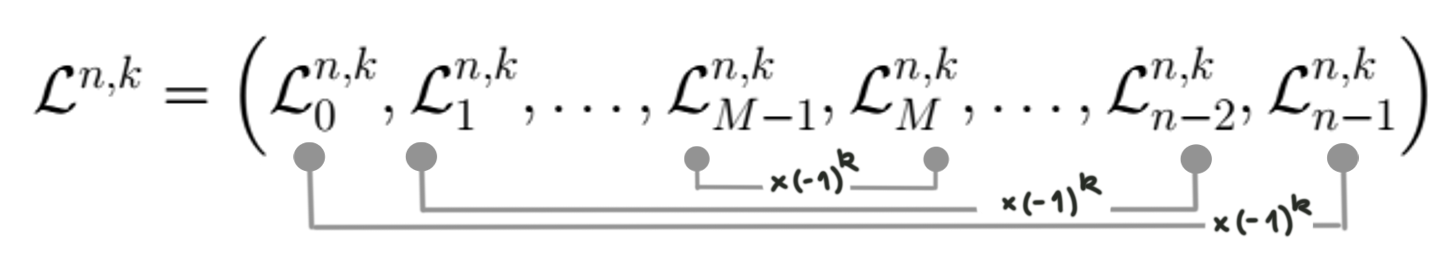
\includegraphics[scale=1.3]{simetria2} 
		\caption{Fijadas una dimensión par $n=2N$ 
		y un grado $0 \leq k \leq n-1$,
		en esta proposición se da una relación simple entre las parejas 
		de entradas de $\cali{L}^{n,m}$ con índices $m$ y $2N-m-1$ 
		(donde los índices $0 \leq m \leq N-1$ son los de las primeras
		$N$ entradas).}
 	\end{measuredfigure}
 \end{figure}

Gracias a lo demostrado en esta sección, sabemos que,
fijada una dimensión $n$ y fijado un grado $0 \leq k \leq n-1$,
el cálculo de las $n$ entradas del vector $\cali{L}^{n,k}$
se reduce al cálculo de la mitad de estas, pues las otras pueden
deducirse de las primeras con un cambio de signo que está completamente
determinado por la paridad del grado $k$.


\begin{figure}[H]
\centering\captionsetup{format = hang}
	\begin{measuredfigure}
		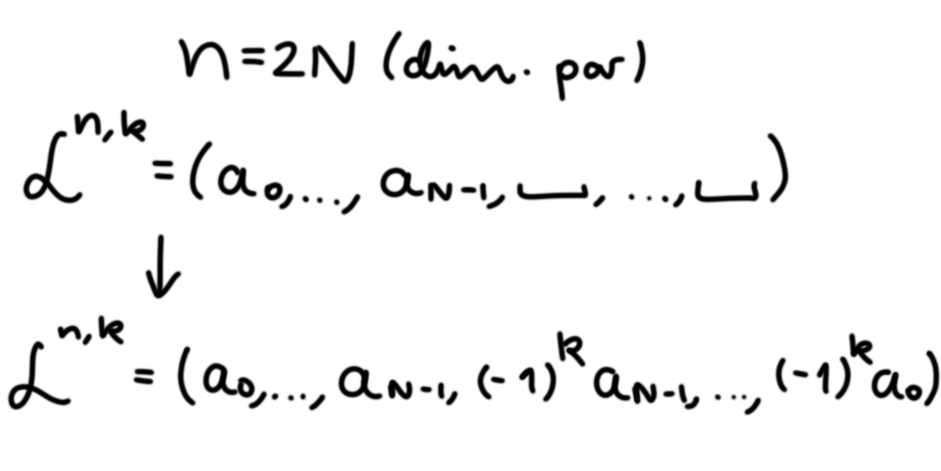
\includegraphics[scale=1]{10Dic_3} 
		\caption{\TODO{aaa}}
 	\end{measuredfigure}
 \end{figure}
